\documentclass[../main.tex]{subfiles}
\graphicspath{{\subfix{../figures/}}}
\begin{document}

\section{$\nu_{\mu}$ CC $\pi^{0}$ Selection}
\label{sec:selection}


\subsection{Signal Definition}
The $\nu_{\mu}$ CC $\pi^{0}$ signal definition encompasses charged-current neutrino interactions occuring within the fiducial volume of the detector and containing
\begin{itemize}
    \item exactly one primary muon
    \item exactly zero charged pions
    \item exactly one neutral pion
    \item any number of particles that are not muons or pions.
\end{itemize}
This signal definition applies to final state particles, or particles exiting the target nucleus post-final state interactions (FSI).  The fiducial volume requirement applies to the neutrino interaction vertex, which must be 25 cm from detector boundaries in the drift and vertical directions, 30 cm from the upstream detector face, and 50 cm from the downstream face.

Additional requirements are placed on the signal definition to ensure tracking thresholds are met and selection purity and efficiency are optimized.  These are referred to as phase space constraints and include:
\begin{itemize}
    \item $p_{\mu} \ge 226$ MeV/c
    \item $p_{\pi^{0}} \ge 100$ MeV/c.
\end{itemize}

\subsection{Selection Cuts}
When selecting $\nu_{\mu}$ CC $\pi^{0}$ interactions, cuts are made on various reconstructed outputs to narrow the list of candidate interactions.  Included are cuts on:
\begin{itemize}
    \item \underline{Fiducial volume}: Reconstructed vertex is required to be inside fiducial volume (defined in signal definition).
    \item \underline{Topology}: Interaction contains exactly one primary muon, zero primary charged pions, and two or three primary photons as reported by the machine-learning reconstruction chain's primary particle classification and particle identification algorithms.  Particles also meet phase space requirements of the signal definition.  In the case of three photons, the pair of photons with reconstructed invariant mass closest to $m_{\pi^{0}}$ is chosen to represent the neutral pion candidate.
    \item \underline{Neutral pion mass}: Invariant diphoton mass $<$ 400 MeV in order to reject $\eta$ mesons.
    \item \underline{Flash time}: Interaction is associated with an optical flash that is in-time with BNB beam gate, as determined by the OpT0Finder algorithm.
\end{itemize}

\subsection{Selection Performance}
Selection performance is assessed using the BNB $\nu$ + Cosmic MC sample and off-beam BNB Run 2 data.  The metrics that have been evaulated are efficiency - the fraction of true signal interactions that are matched to selected interactions, and purity - the fraction of selected interactions that are matched to true signal interactions.  Figure \ref{fig:prephase_efficiency} shows the selection efficiency for $\nu_{\mu}$ CC $\pi^{0}$ events before muon and neutral pion momentum thresholds are applied.  The sharp drop-offs at 226 MeV/c and 100 MeV/c for the muon and neutral pion distributions, respectively, motivate the phase space constraints of the signal definition.


\begin{figure}[H]
    \center
    \subfloat{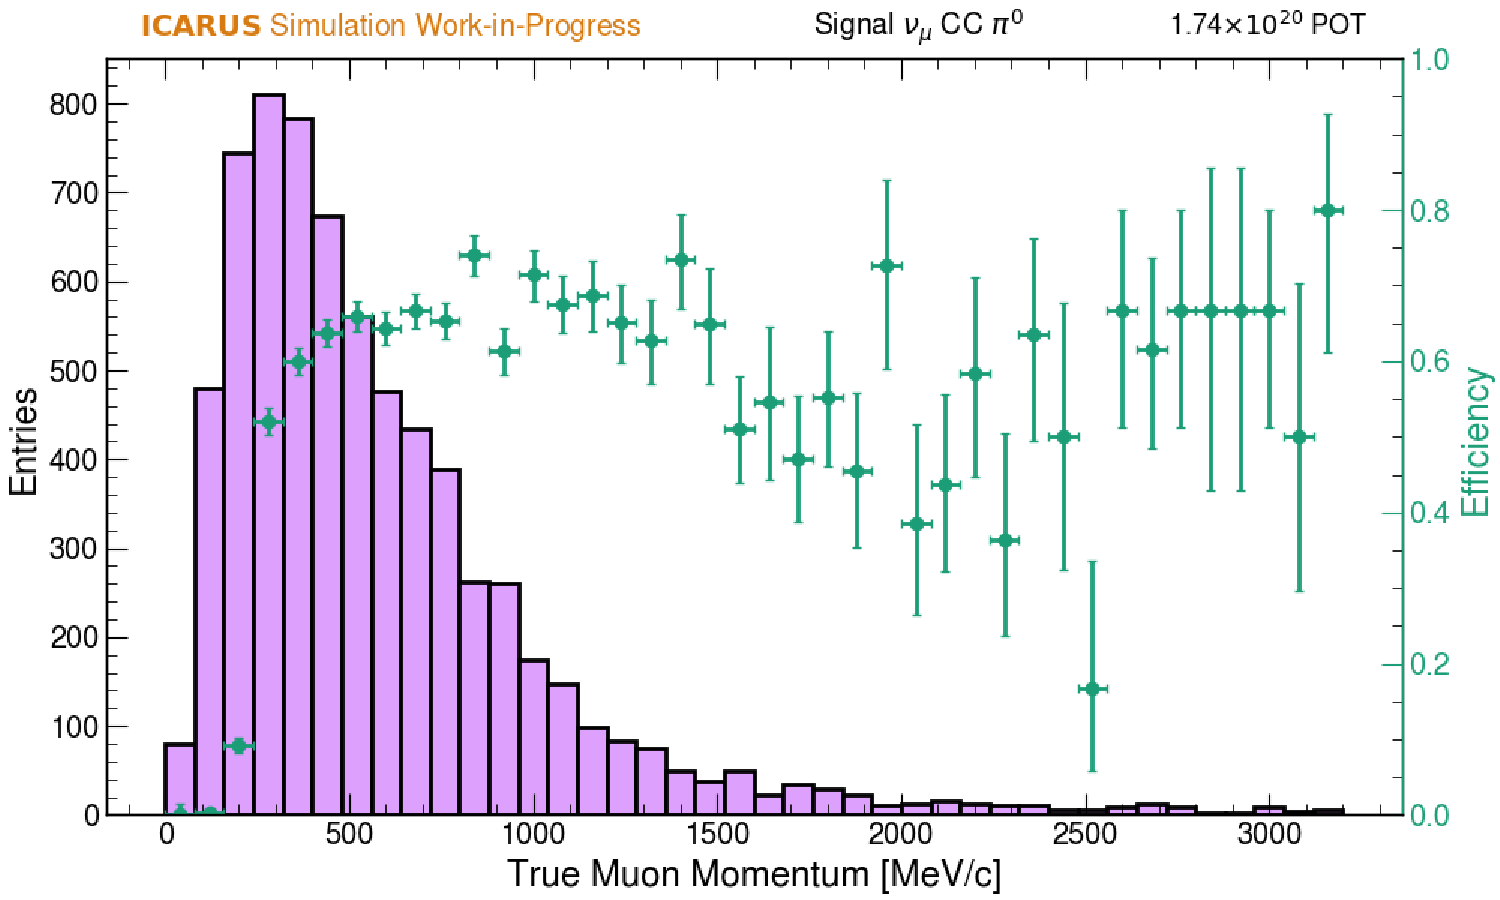
\includegraphics[width=0.90\textwidth]{eff_vs_muon_momentum_mag.pdf}}\\

    \subfloat{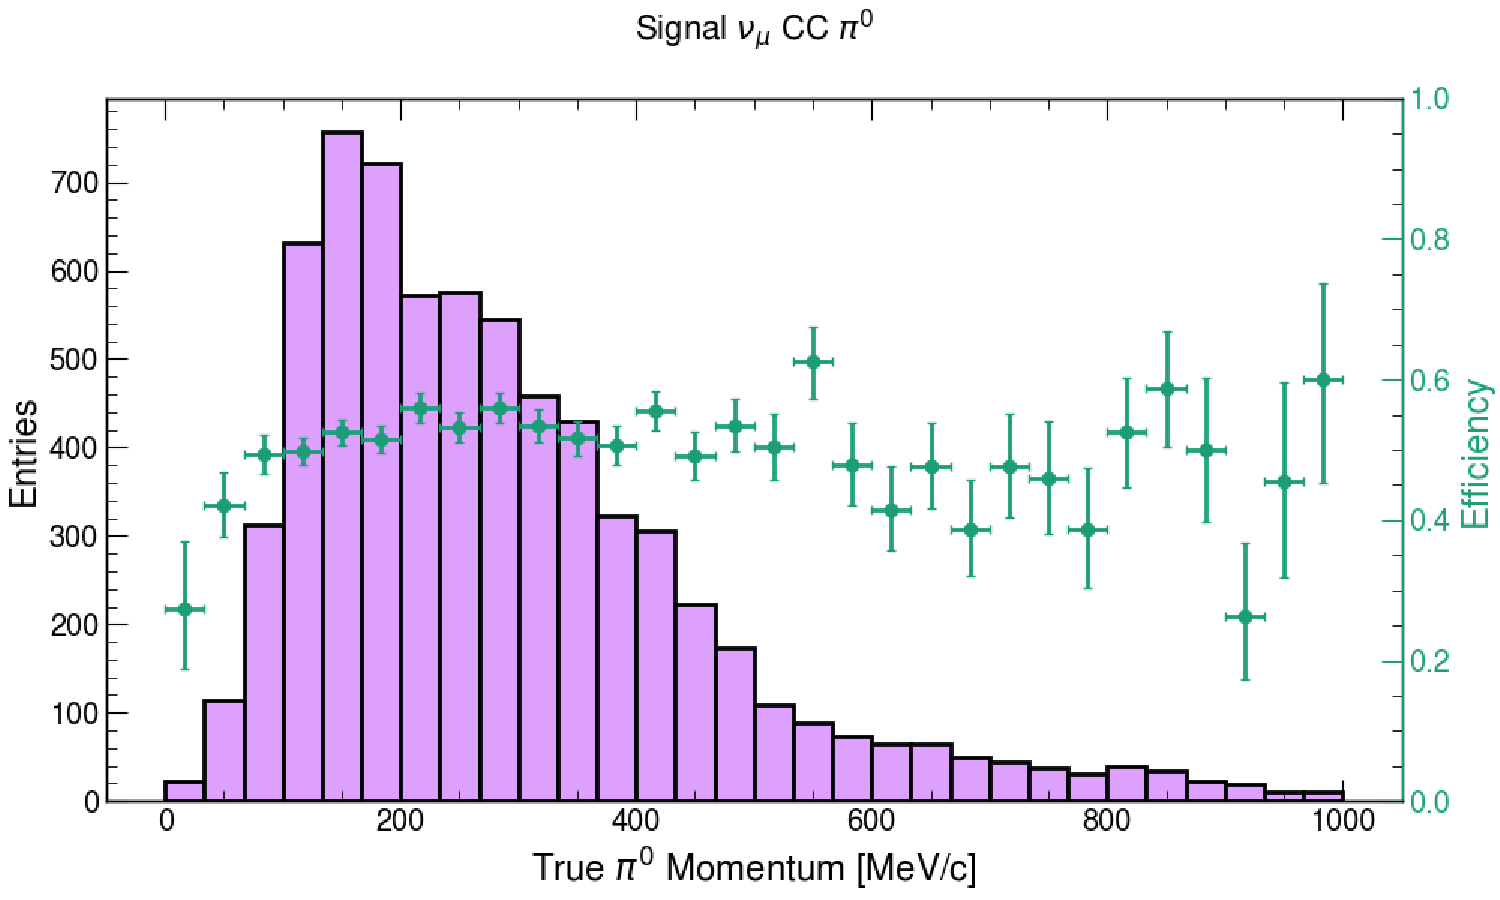
\includegraphics[width=0.90\textwidth]{eff_vs_pi0_momentum_mag.pdf}} 

    \caption{Efficiency of selecting signal events as a function of muon and neutral pion momentum.}
    \label{fig:prephase_efficiency}
\end{figure}

After phase space constraints are placed, the selection achieves an efficiency of 59.68\% and a purity of 84.33\%.   Efficiency and purity for each selection cut are shown in Table \ref{Tab:pureff}.  Inefficiencies and impurities are primarily driven by PID failures, which are further characterized in \ref{fig:sel_pid_confusion}.  Background topologies can also be seen in Section \ref{subsec:vars}.

\begin{table}[ht]
    \caption{Purity and efficiency for $\nu_{\mu}$ CC $\pi^{0}$ Selection Cuts}
    \vspace{0.1cm}
    \centering
    \begin{tabular}{ c c c } 
    \hline
    Selection Cut & Efficiency [\%] & Purity [\%]  \\
    \hline
    No Cut & 100 & 0.09 \\ 
    In-Time Flash & 96.6 & 2.64 \\
    Fiducial Volume & 95.73 & 4.03 \\
    Topology & 59.77 & 83.18 \\
    $m_{\gamma \gamma} < 400$ MeV/c$^{2}$ & 59.68 & 84.33 \\
    \hline
    \end{tabular}
    \label{Tab:pureff}
\end{table}

\begin{figure}[H]
    \center
    \subfloat[True-to-reco matching.]{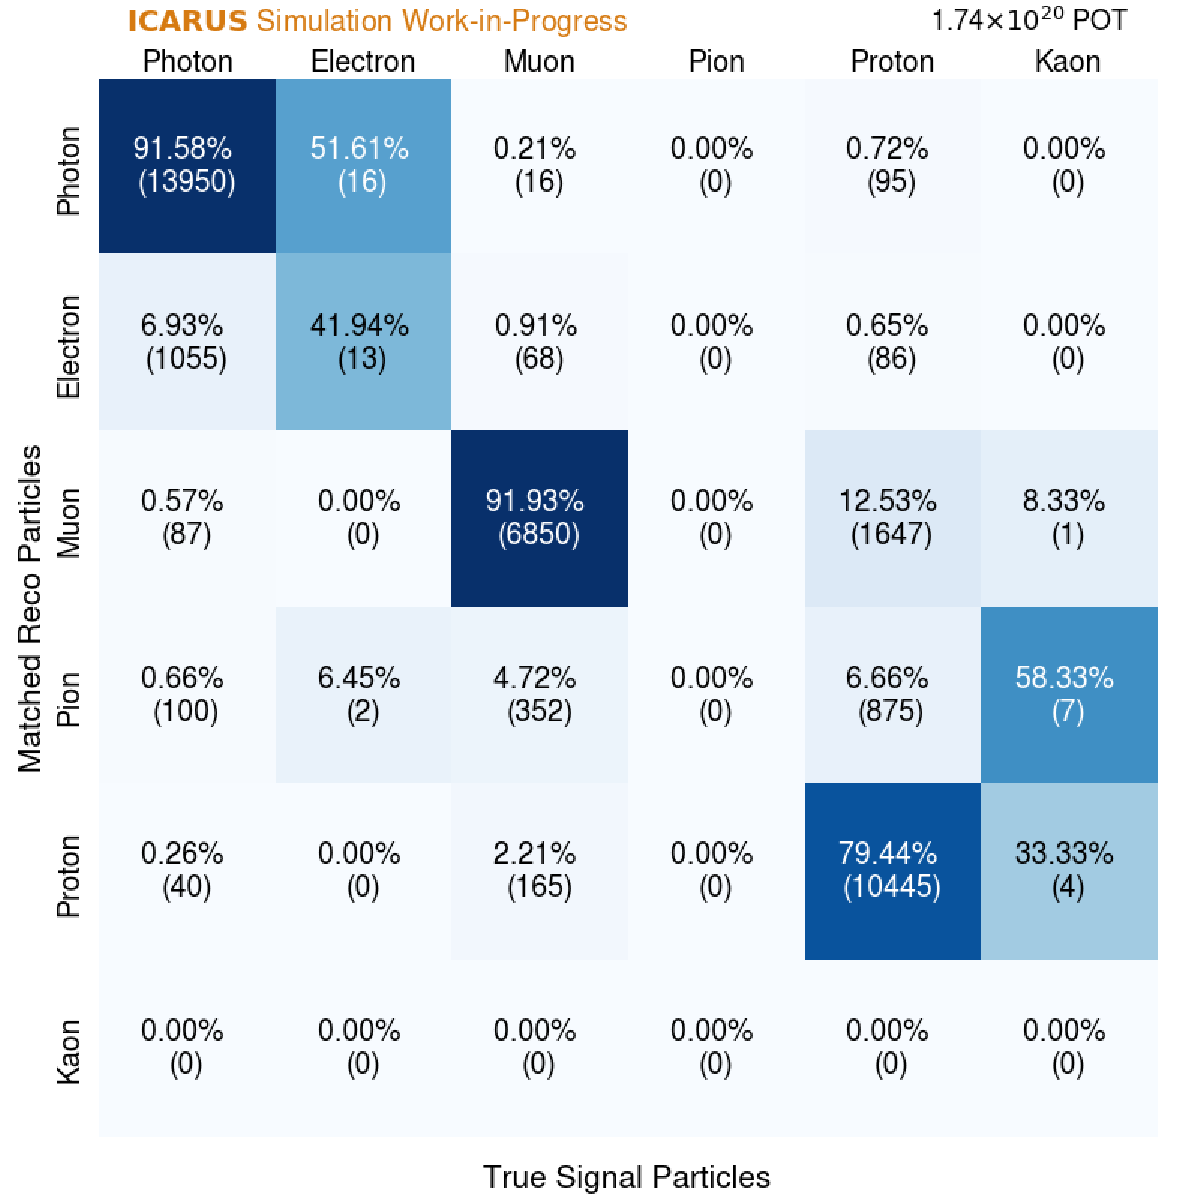
\includegraphics[width=0.50\textwidth]{eff_pid_confusion.pdf}}
    \subfloat[Reco-to-true matching.]{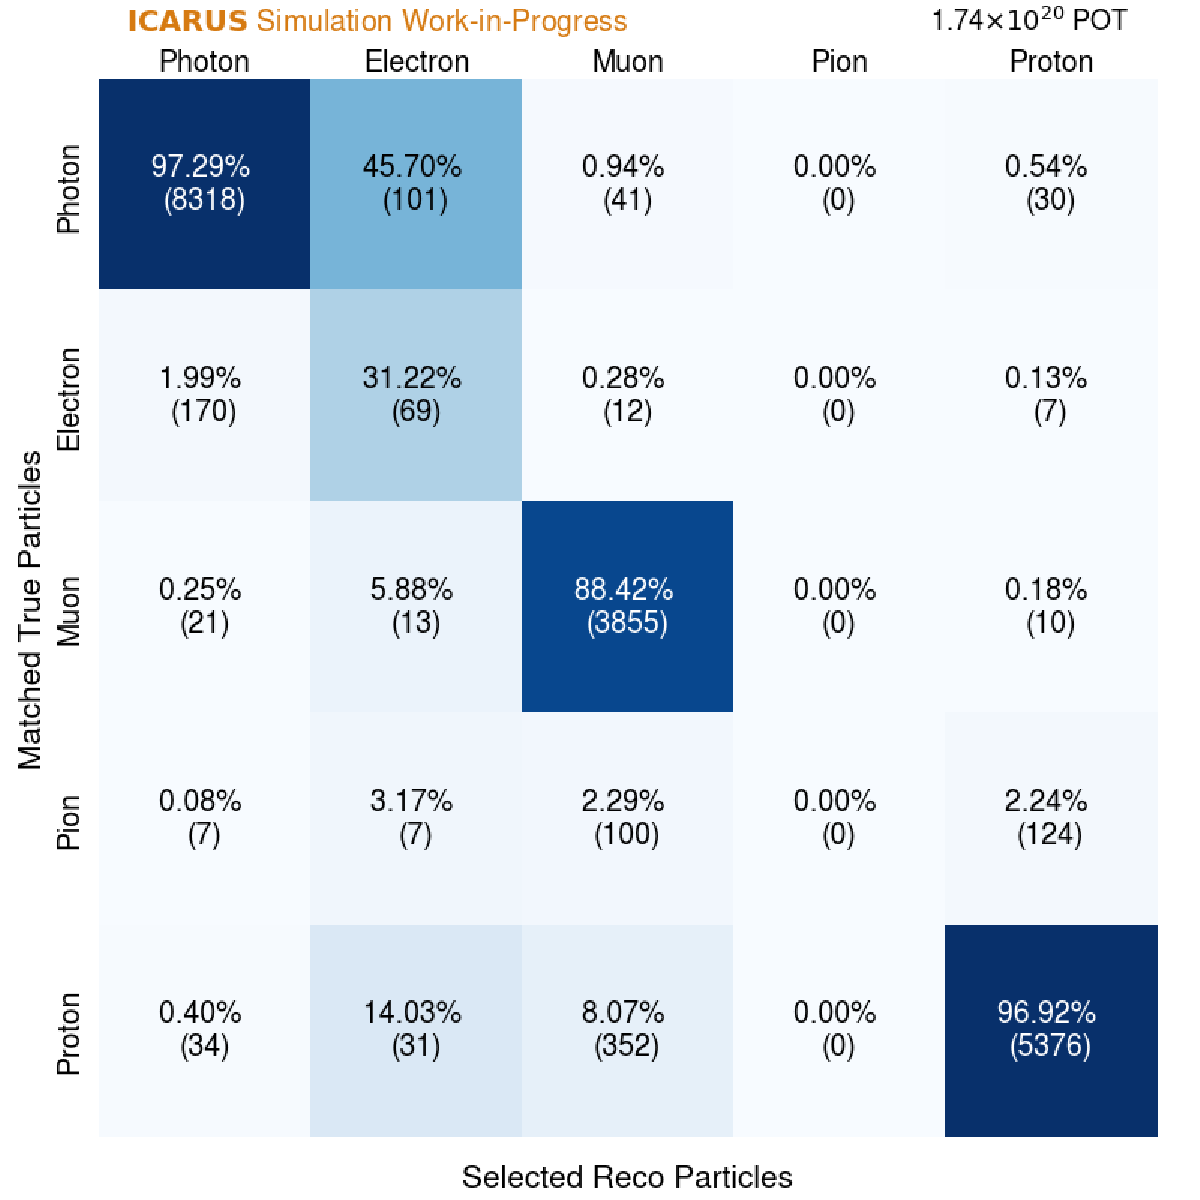
\includegraphics[width=0.50\textwidth]{pur_pid_confusion.pdf}} 
    \caption{Confusion matrices for particle identification, as determined by the SPINE machine-learning chain.}
    \label{fig:sel_pid_confusion}
\end{figure}

\subsection{Variables of Interest}
\label{subsec:vars}
In this section, the kinematic observables used in the single differential cross section measurement are discussed.  Included are the momenta of the final state muon and neutral pion, as well as the angles these particles make with the BNB.  An additional variable, the invariant diphoton mass, is examined as it serves as a useful standard candle in the calibration of the electromagnetic shower energy scale.  First, however, the methods used to estimate the energy (and momentum) of the reconstructed particles of interest is detailed.

\subsubsection{Energy Reconstruction}
To estimate the momentum of the reconstructed muon, it is first necessary to reconstruct its energy, for which a ``best estimate" approach is taken.  For muons contained within the active detector volume, momentum is calculated using the Continous Slowing Down Approximation (CSDA) that relates a particle's kinetic energy to its range in a material.  For momentum estimation of exiting muons, the degree of multiple coulomb scattering (MCS) along the track is instead used.  Figure \ref{fig:muon_energy} shows how each muon momentum estimate compares with true muon momentum in simulation.

\begin{figure}[H]
    \center
    \subfloat[Range-based energy reconstruction.]{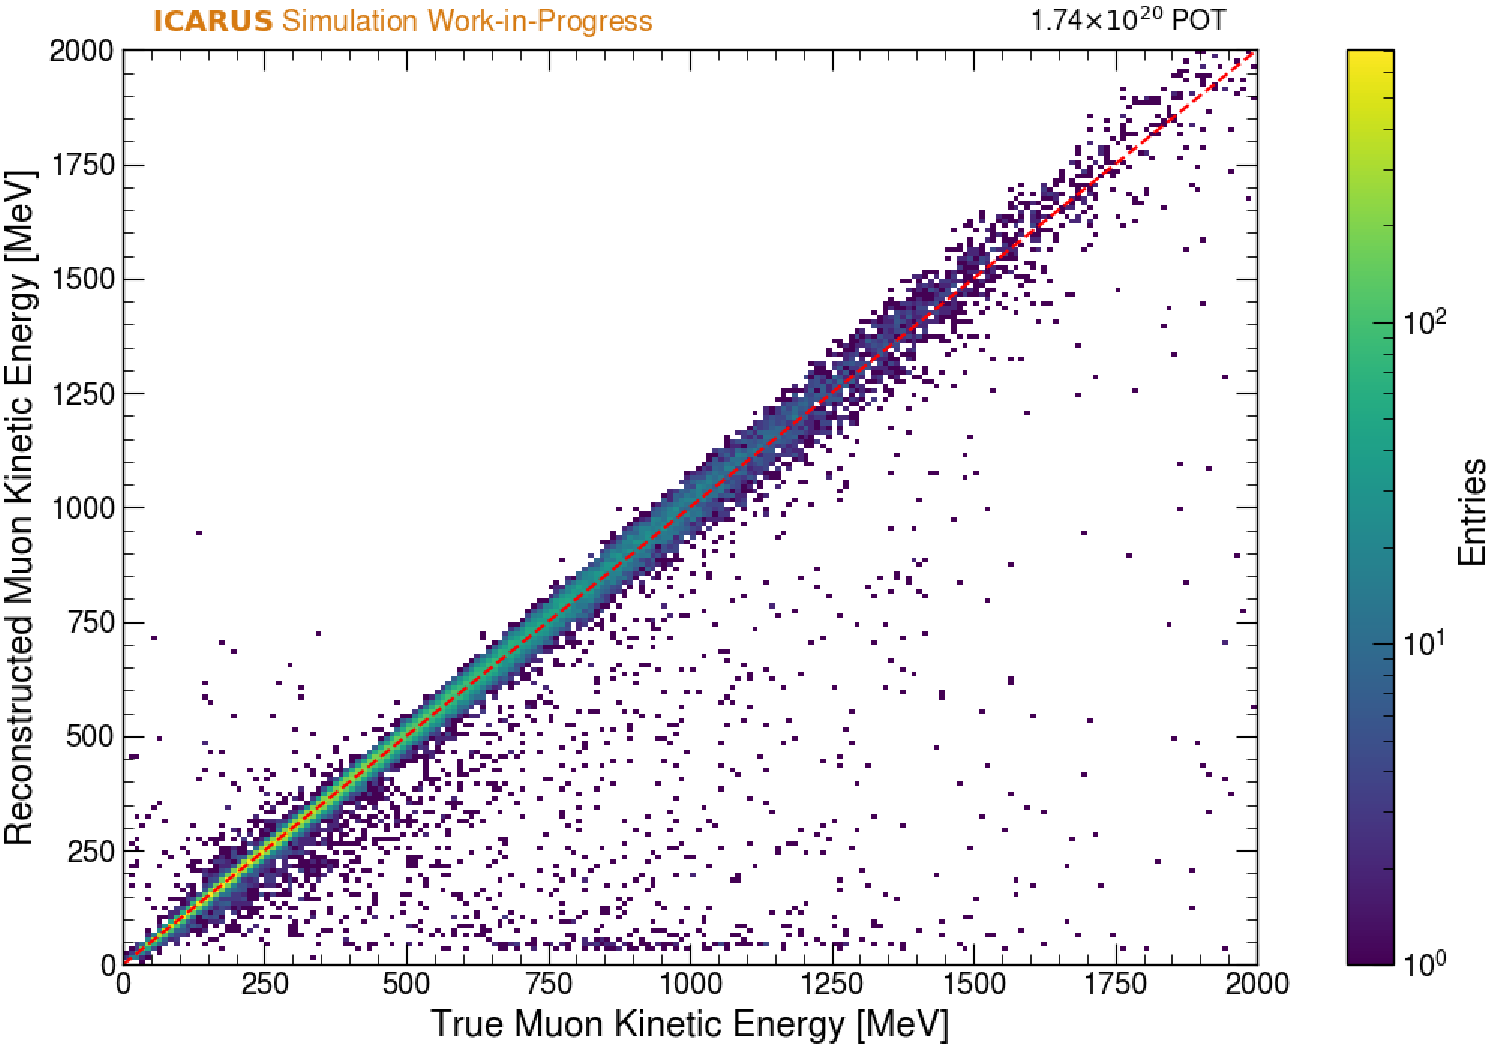
\includegraphics[width=0.50\textwidth]{muon_reco_csda_ke_vs_true_ke.pdf}}
    \subfloat[Multiple coulomb scatering-based energy reconstruction.]{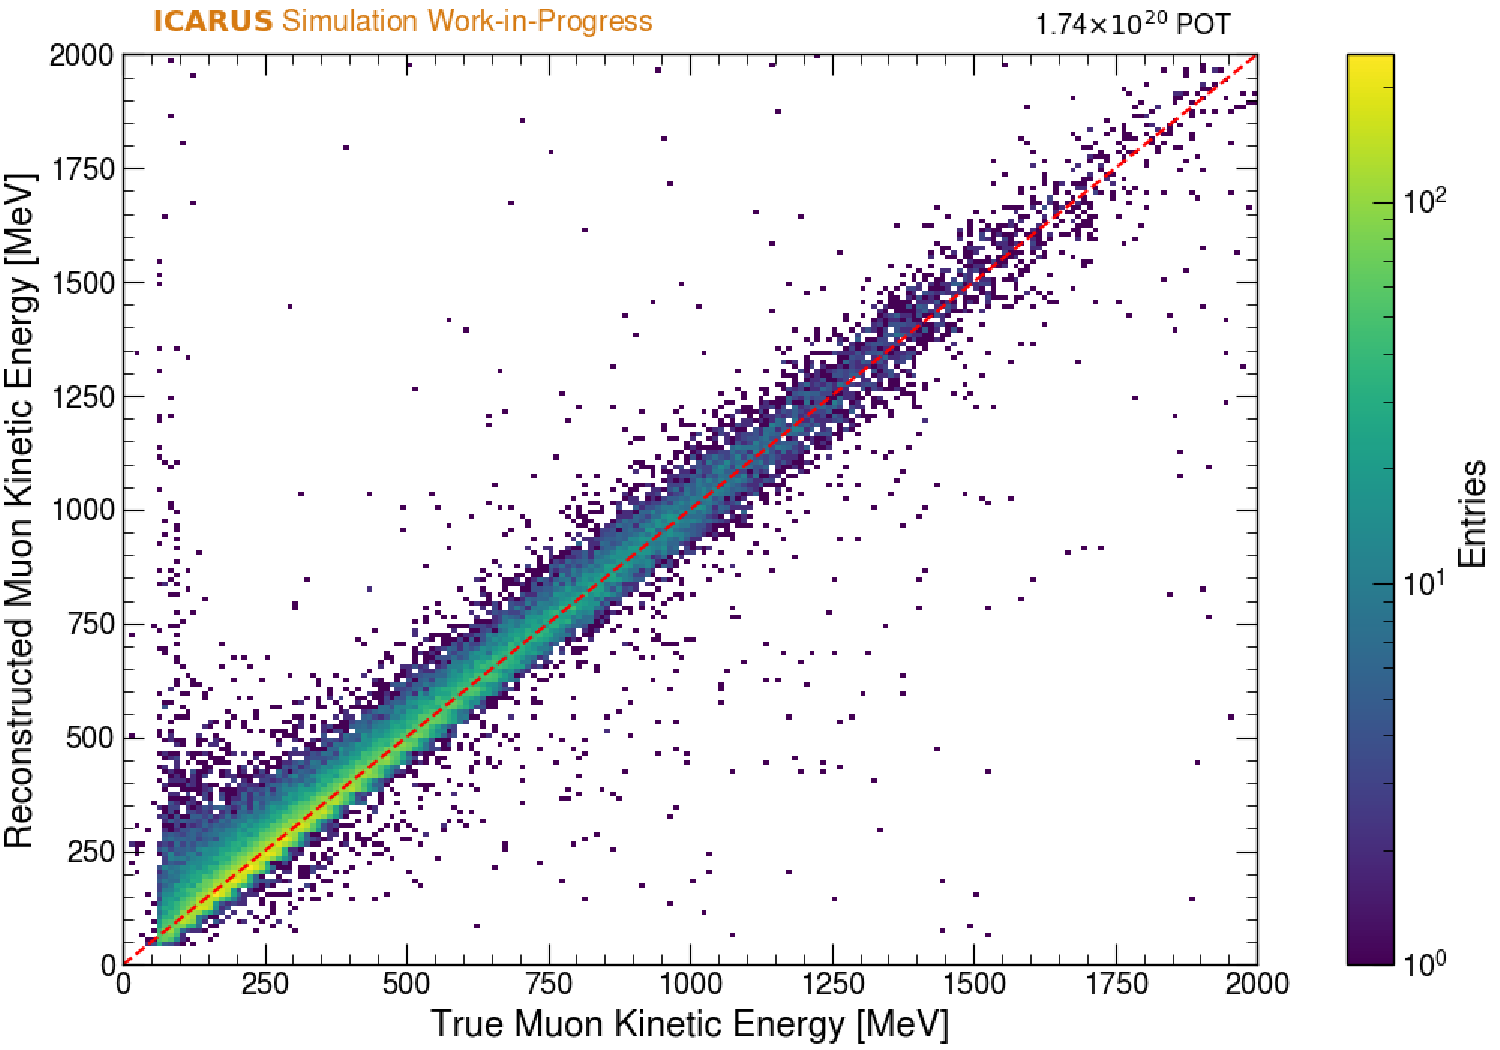
\includegraphics[width=0.50\textwidth]{muon_reco_mcs_ke_vs_true_ke.pdf}} 
    \caption{Comparisons of reconstructed and true muon kinetic energy for a selection of contained muons in ICARUS simulation.}
    \label{fig:muon_energy}
\end{figure}

Unlike muons, neutral pions do not directly ionize the detector medium.  The neutral pion momentum must therefore be inferred from the electromagnetic showers instigated by the photons it decays to.  Shower energy (and momentum) is estimated calorimetrically by summing charge depositions belonging to the shower and accounting for various detector effects:
\begin{equation}
    E_{shower} = W_{i} [\frac{MeV}{e^{-}}] \cdot C_{cal} [\frac{e^{-}}{ADC}] \cdot C_{adj} \cdot \frac{1}{R} \cdot \sum_{dep} e^{\frac{t_{drift}}{\tau}} \cdot dep [ADC],
    \label{eq:shower_energy}
\end{equation}
where
\begin{itemize}[label=]
    \setlength\itemsep{0.1ex}
    \item $W_{i}$ is the work function for argon
    \item $C_{cal}$ converts charge units from ADC to electrons
    \item $C_{adj}$ accounts for missing energy due to subthreshold charge and clustering effects in reconstruction
    \item $R$ is the recombination factor
    \item $\tau$ is the electron lifetime
    \item $dep$ is charge in units of ADC.
\end{itemize}

The shower correction factor, $C_{adj}$, is derived from a study of contained photons in simulation.  Figure \ref{subfig:shower_correction} shows the ratio of reconstructed photon energy (from equation \ref{eq:shower_energy}) to true photon energy.  As this ratio is mostly flat across different energies, a constant correction factor is chosen.  Reconstructed photon energy is again compared to true photon energy in \ref{subfig:photon_reco_vs_true_energy}, showing agreement after the correction factor is applied.  It is also worth noting that since the analyis signal definition does not require showers to be contained, an additional correction factor is needed to correct for missing energy in exiting showers.  A study for deriving this factor is ongoing with results expected soon.

\begin{figure}[H]
    \center
    \subfloat[Shower correction factor]
        {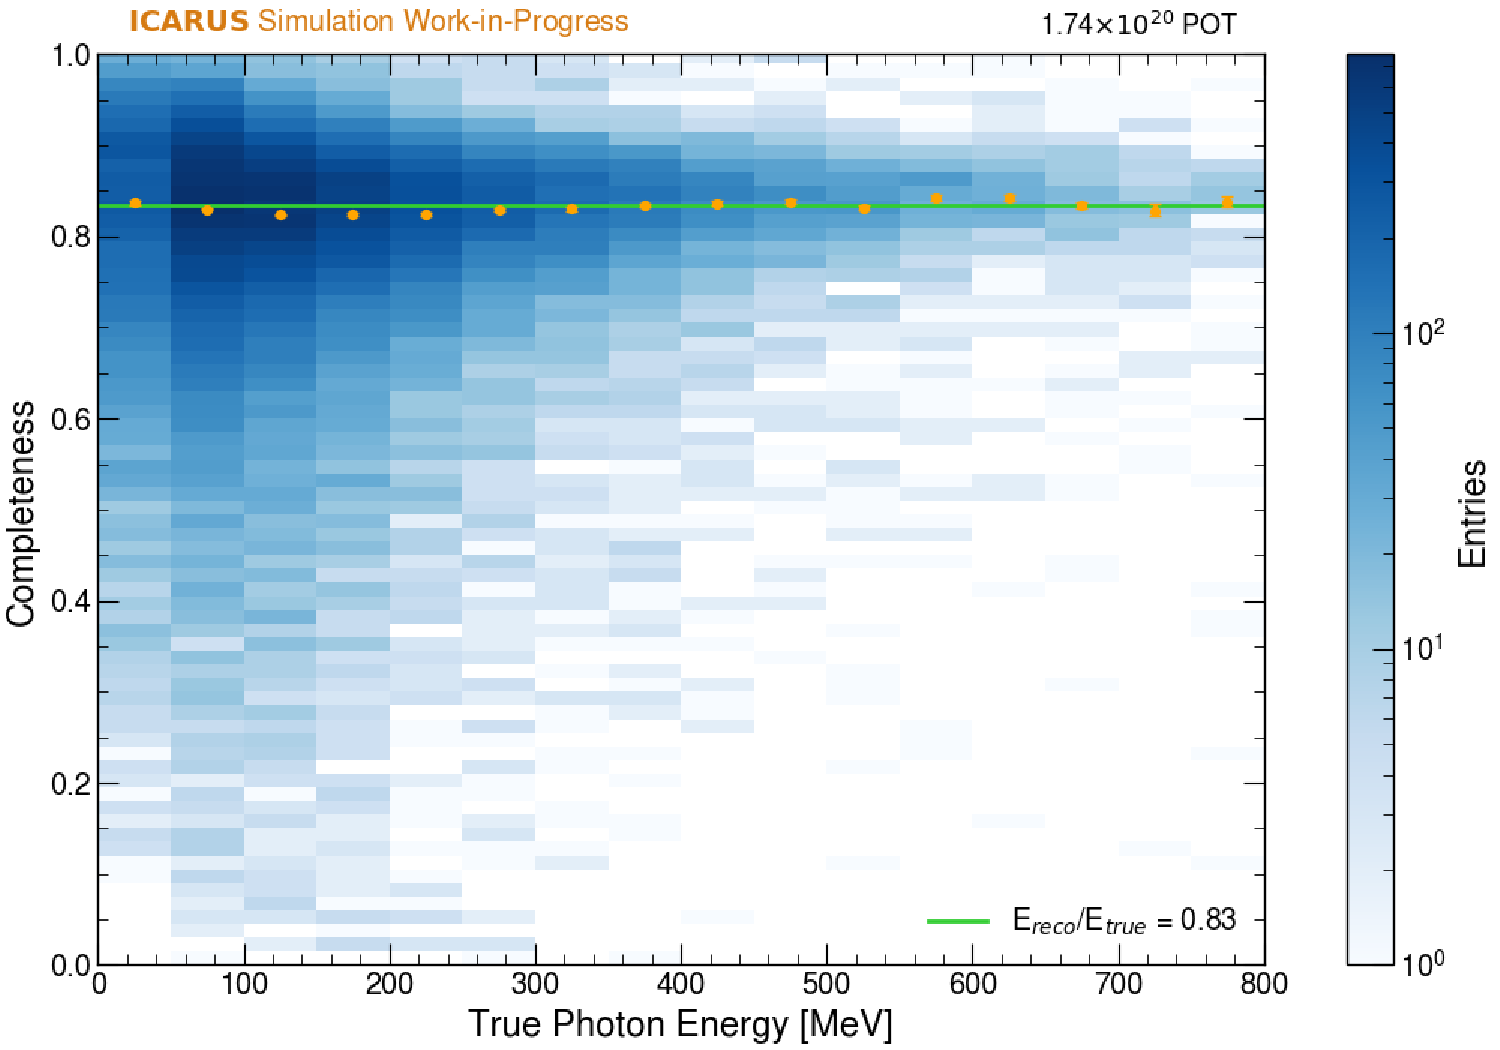
\includegraphics[width=0.50\textwidth]{shower_corr.pdf} \label{subfig:shower_correction}}
    \subfloat[Comparison of reconstructed and true photon energies after correction is applied]
        {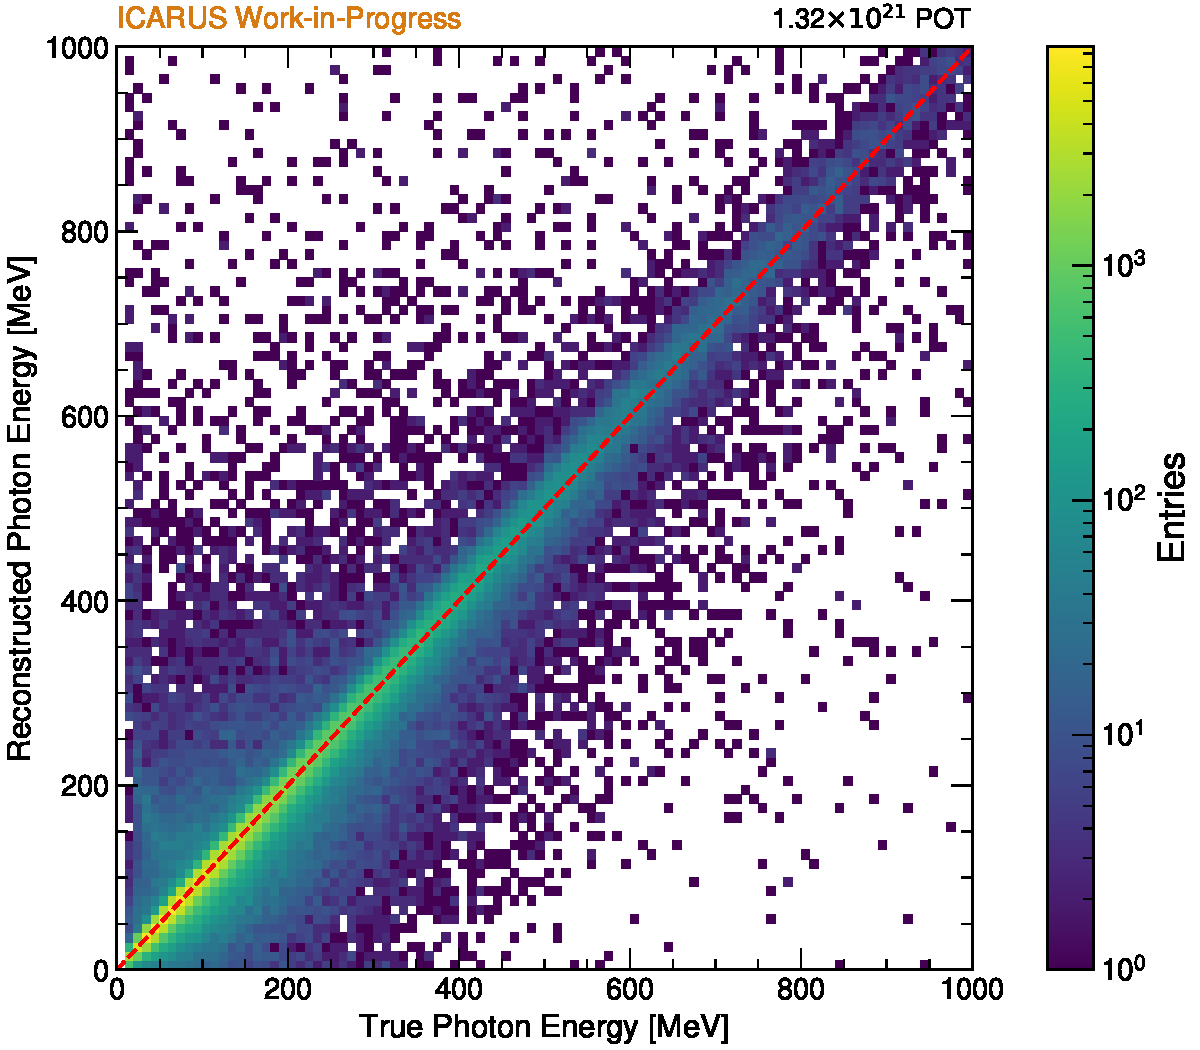
\includegraphics[width=0.50\textwidth]{photon_reco_vs_true_energy.pdf} \label{subfig:photon_reco_vs_true_energy}}
    \caption{Study of reconstructed electromagnetic shower energy.}
    \label{fig:photon_energy}
\end{figure}

\subsubsection{Muon Observables}
\begin{figure}[H]
    \center
    \subfloat[Muon momentum]
        {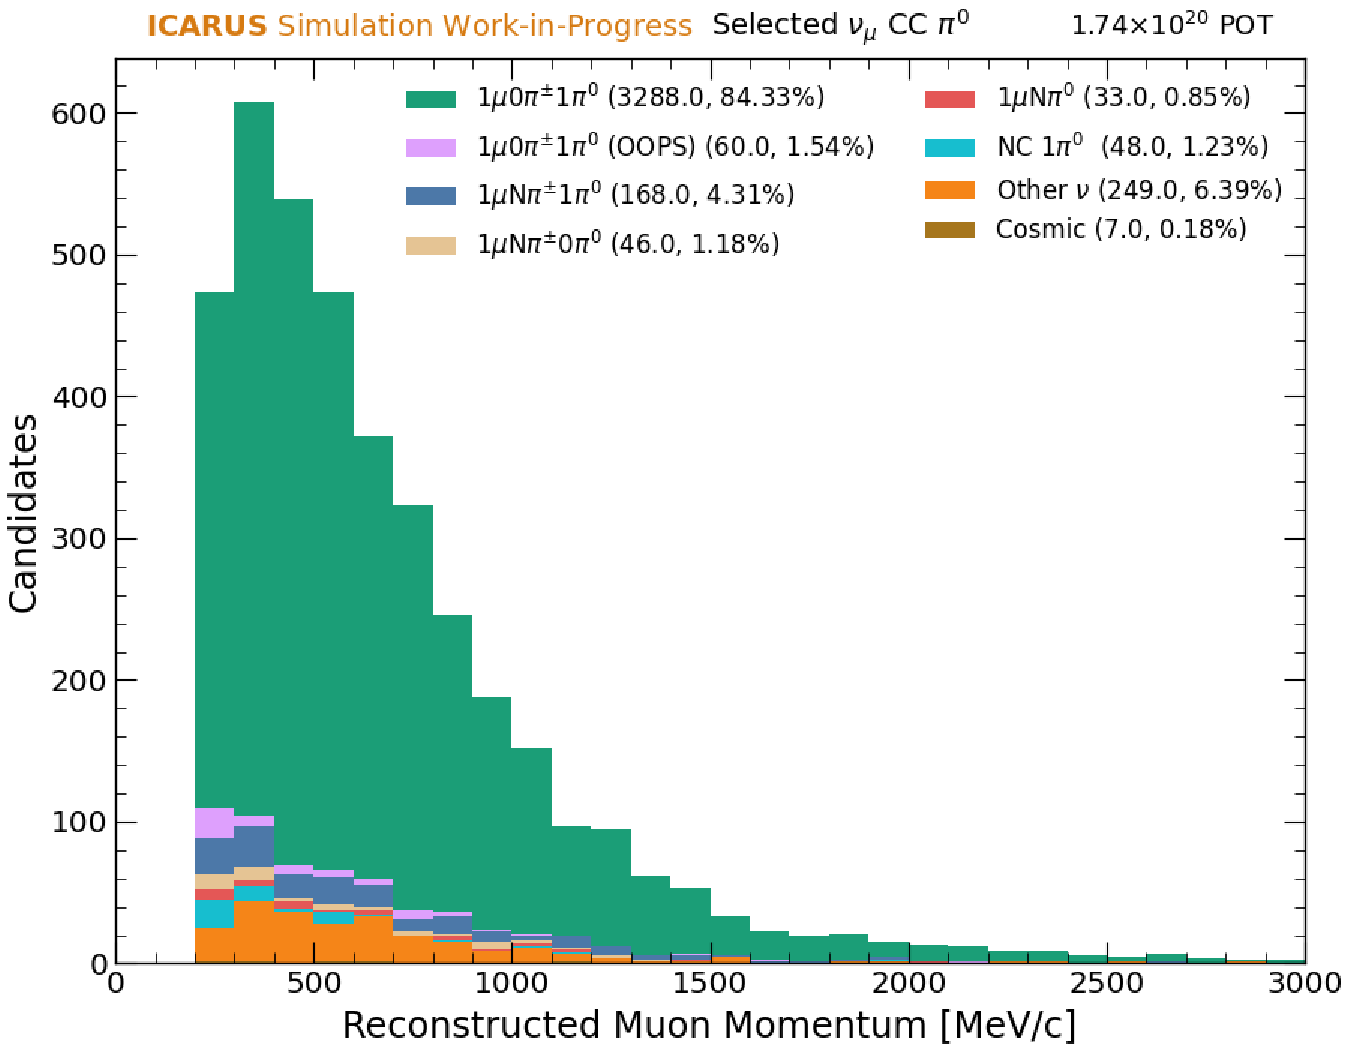
\includegraphics[width=0.50\textwidth]{muon_momentum_mag_mc.pdf} \label{subfig:muon_momentum_mag_mc}}
    \subfloat[Muon angle with respect to neutrino]
        {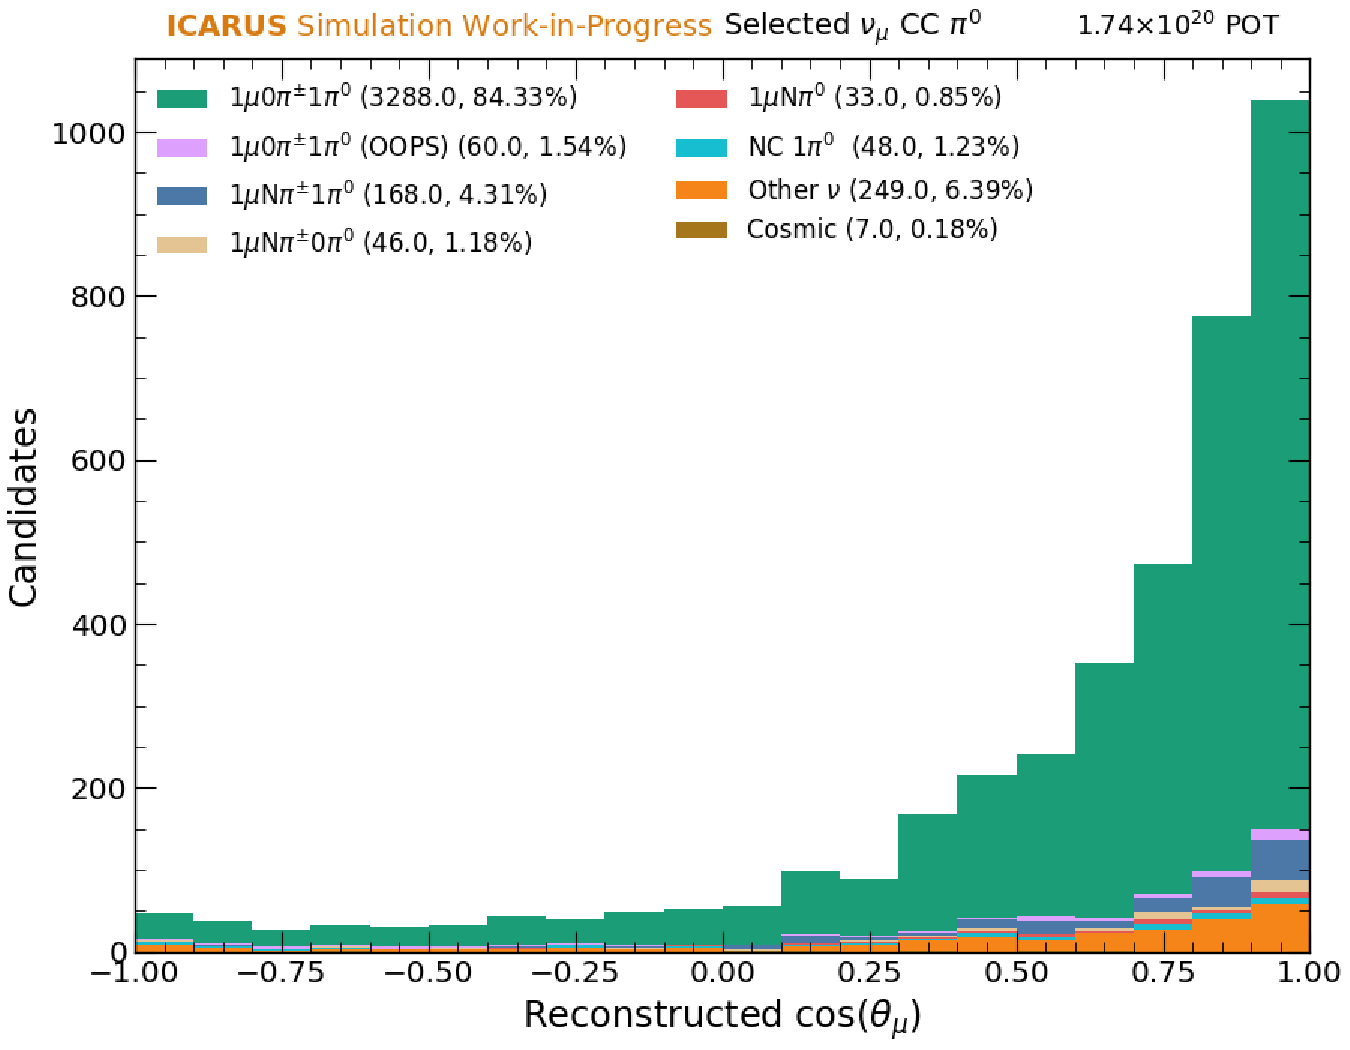
\includegraphics[width=0.50\textwidth]{muon_beam_costheta_mc.pdf} \label{subfig:muon_beam_costheta_mc}}
    \caption{Muon observables chosen for analysis}
    \label{fig:muon_observables_mc}
\end{figure}

\subsubsection{Photon Observables}
\begin{figure}[H]
    \center
    \subfloat[Subleading Photon Energy]
        {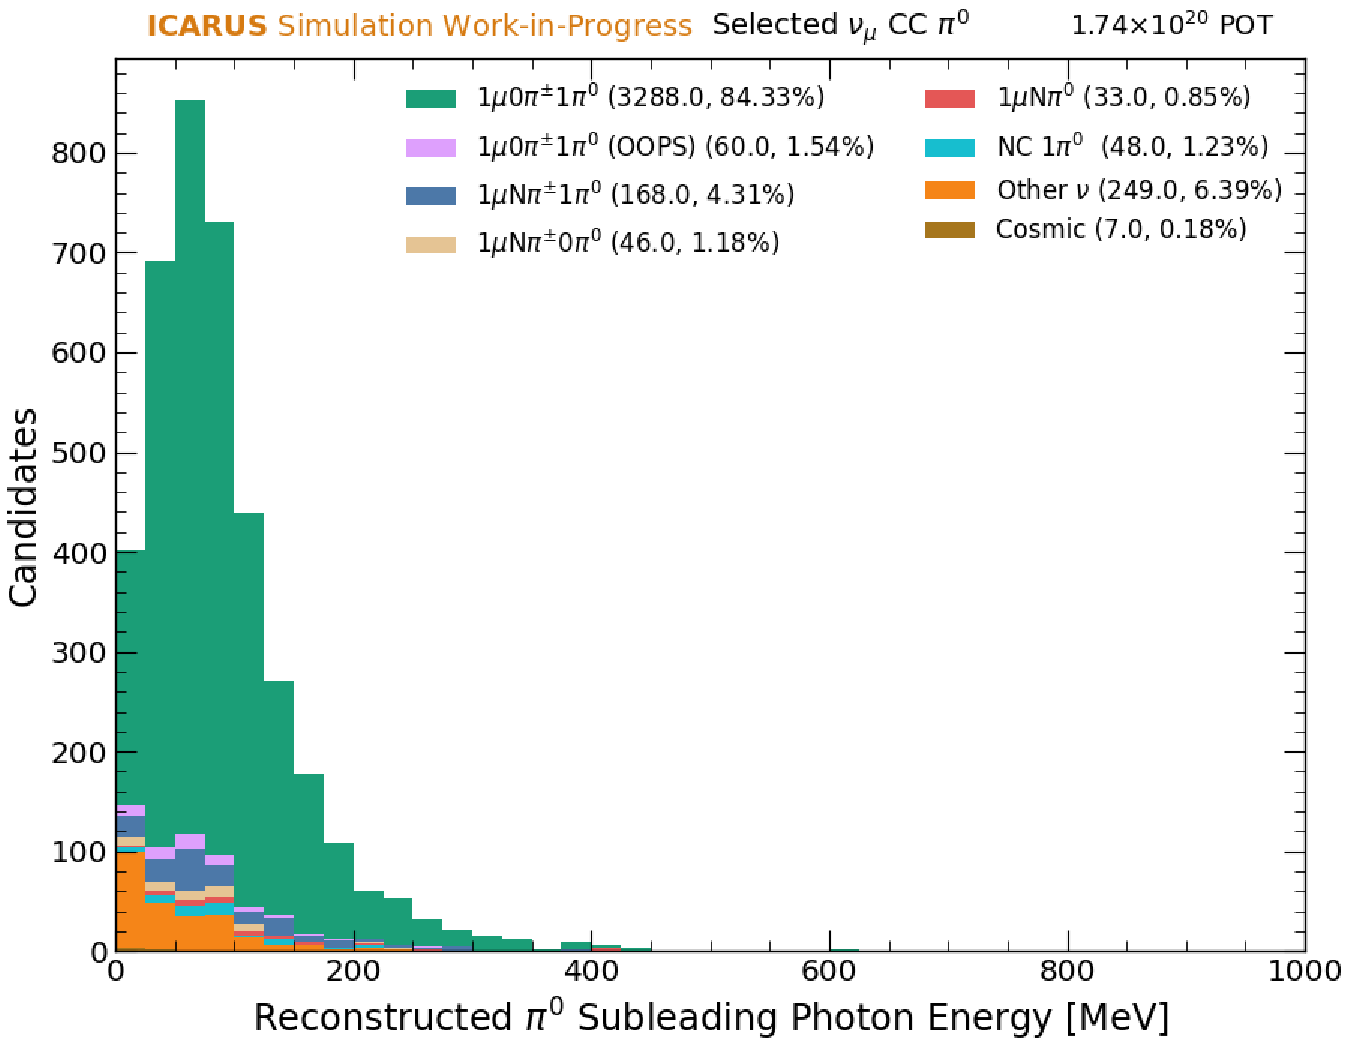
\includegraphics[width=0.50\textwidth]{pi0_subleading_photon_energy_mc.pdf} \label{subfig:pi0_subleading_photon_energy_mc}}
    \subfloat[Leading Photon Energy]
        {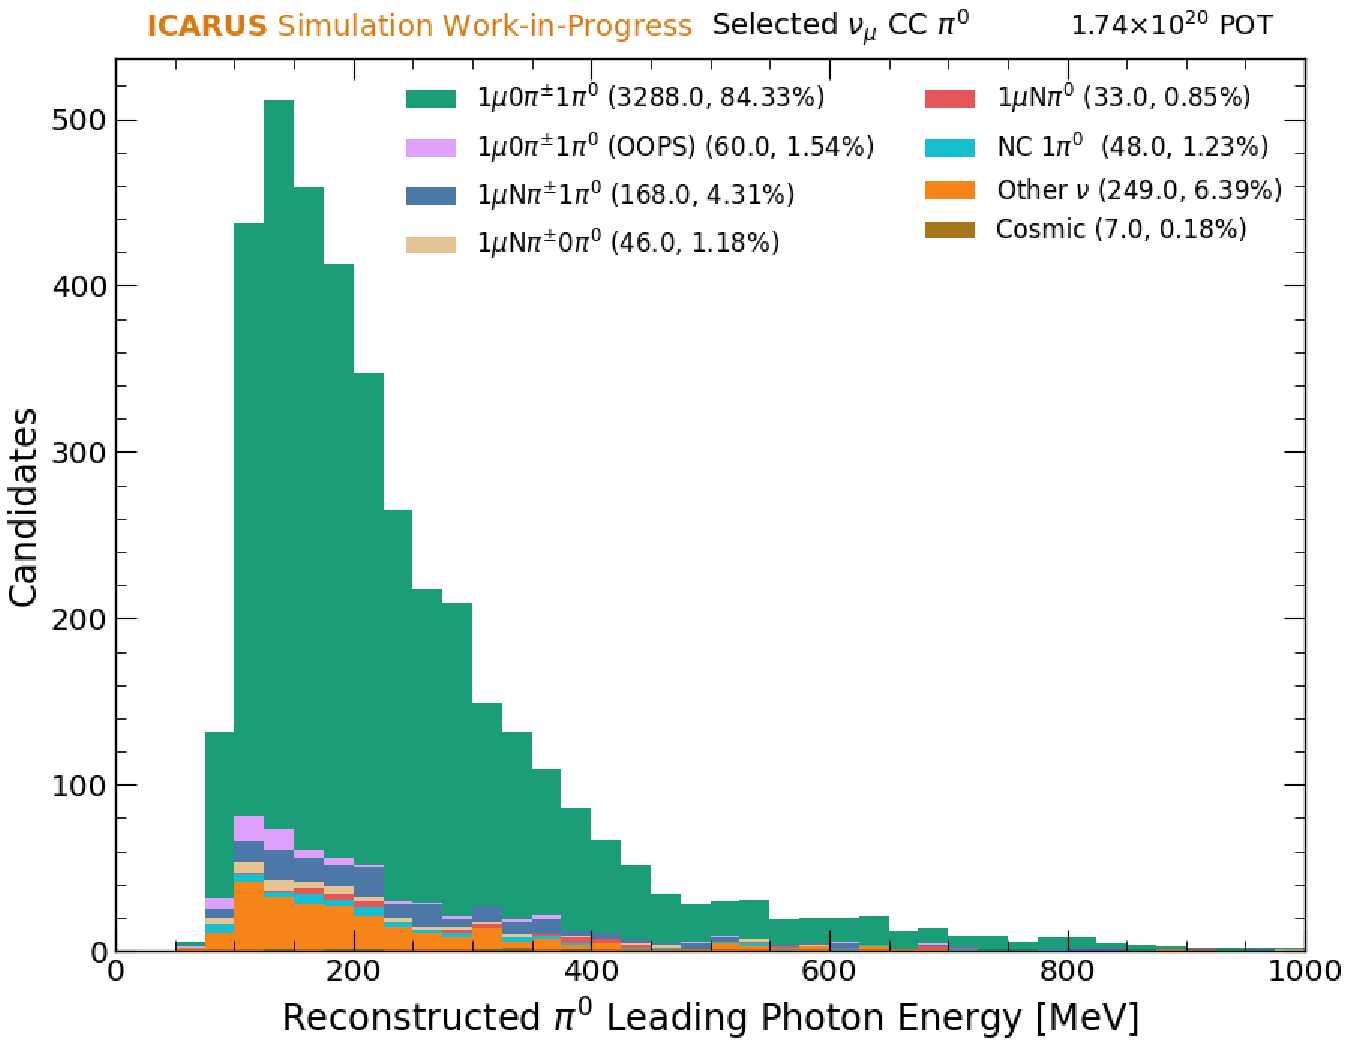
\includegraphics[width=0.50\textwidth]{pi0_leading_photon_energy_mc.pdf} \label{subfig:pi0_leading_photon_energy_mc}}
        
    \subfloat[Subleading Photon Conversion Distance]
        {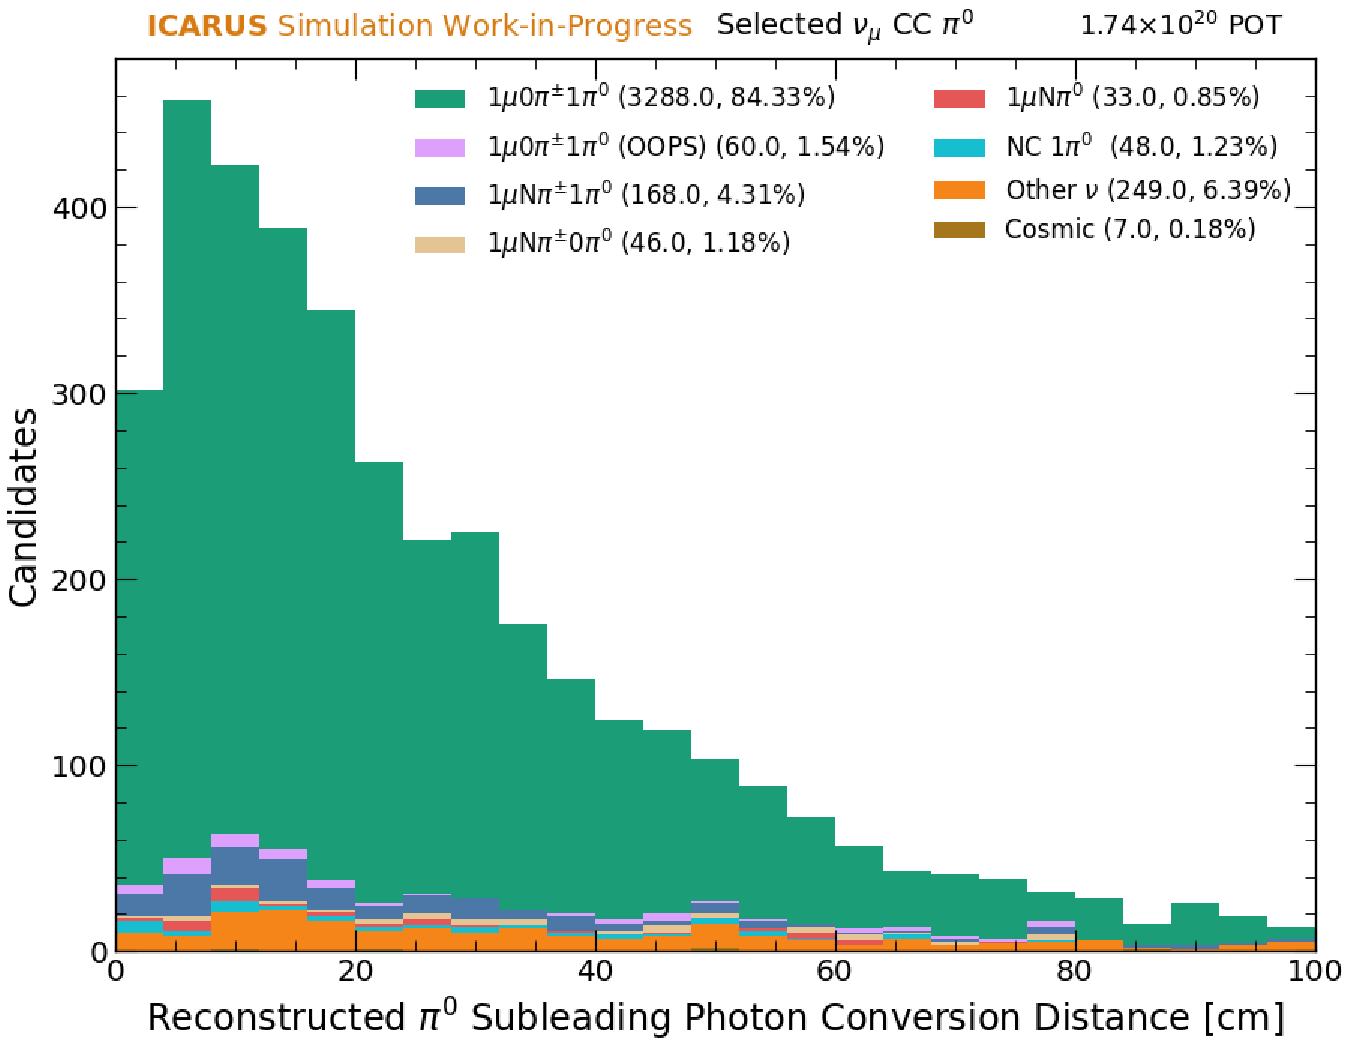
\includegraphics[width=0.50\textwidth]{pi0_subleading_photon_conv_dist_mc.pdf} \label{subfig:pi0_subleading_photon_conv_dist_mc}}
    \subfloat[Leading Photon Conversion Distance]
        {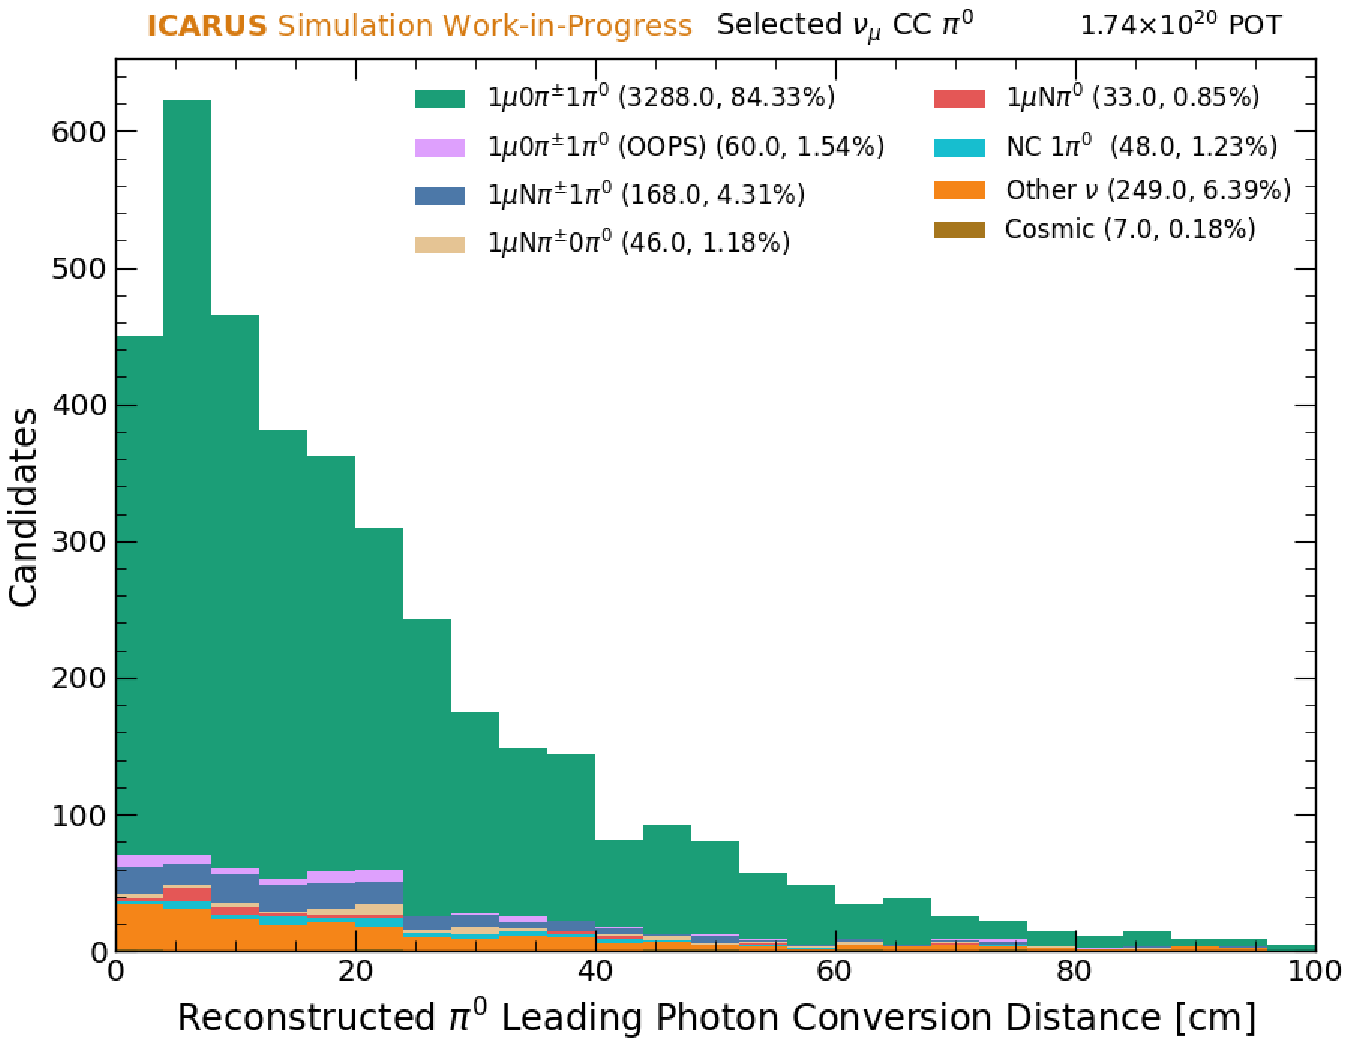
\includegraphics[width=0.50\textwidth]{pi0_leading_photon_conv_dist_mc.pdf} \label{subfig:pi0_leading_photon_conv_dist_mc}}        
    \caption{Photon observables chosen for analysis (not directly used in cross section measurement)}
    \label{fig:photon_observables_mc}
\end{figure}

\subsubsection{Neutral Pion Observables}
\begin{figure}[H]
    \center
    
\includegraphics[width=0.45\textwidth]{missing.pdf}
    %\hspace{1cm}
    
\includegraphics[width=0.45\textwidth]{missing.pdf}
    \caption[text]{A missing figure.}
    \label{fig:pi0_obs0}
\end{figure}

\begin{figure}[H]
    \center
    
\includegraphics[width=0.90\textwidth]{missing.pdf}
    \caption[text]{A missing figure.}
    \label{fig:pi0_obs1}
\end{figure}


\end{document}